\documentclass[12pt,a4paper]{article}
\usepackage[utf8]{inputenc}
\usepackage[T1]{fontenc}
\usepackage{graphicx}
\usepackage{hyperref}
\usepackage{geometry}
\usepackage{fancyhdr}
\usepackage{titlesec}
\usepackage{amsmath}
\usepackage{amssymb}
\usepackage{xcolor}
\usepackage{listings}
\usepackage{tikz}
\usetikzlibrary{shapes,arrows,positioning,calc}

% DFD Styles
\tikzset{
    entity/.style={
        draw=corporate-primary,
        fill=corporate-bg,
        rectangle,
        thick,
        minimum width=2.5cm,
        minimum height=1.2cm,
        font=\small\bfseries,
        inner sep=5pt
    },
    process/.style={
        draw=corporate-primary,
        fill=corporate-bg,
        rounded corners=10pt,
        thick,
        minimum width=3.5cm,
        minimum height=1.8cm,
        font=\large\bfseries\color{corporate-primary},
        align=center
    },
    datastore/.style={
        draw=corporate-secondary,
        thick,
        shape=rectangle,
        minimum width=2cm,
        minimum height=0.8cm,
        font=\small\itshape,
        append after command={
            \pgfextra{
                \draw[thick, corporate-secondary] (\tikzlastnode.north west) -- (\tikzlastnode.north east);
                \draw[thick, corporate-secondary] (\tikzlastnode.south west) -- (\tikzlastnode.south east);
            }
        }
    },
    flow/.style={
        ->,
        >=stealth,
        thick,
        color=corporate-secondary,
        font=\scriptsize,
        shorten >=1pt,
        text centered
    }
}

\geometry{margin=1in}

\definecolor{corporate-primary}{RGB}{30,58,138}    % Deep Blue / Indigo
\definecolor{corporate-secondary}{RGB}{71,85,105} % Slate Gray
\definecolor{corporate-accent}{RGB}{59,130,246}  % Bright Blue
\definecolor{corporate-bg}{RGB}{248,250,252}      % Soft Background
\definecolor{corporate-success}{RGB}{21,128,61}   % Muted Green
\definecolor{corporate-warning}{RGB}{194,65,12}   % Muted Orange
\definecolor{corporate-border}{RGB}{203,213,225}    % Soft Border

\hypersetup{colorlinks=true, linkcolor=corporate-primary, filecolor=magenta, urlcolor=corporate-accent}

\titleformat{\section}{\normalfont\Large\bfseries\color{corporate-primary}}{}{0pt}{\thesection. }
\titleformat{\subsection}{\normalfont\large\bfseries\color{corporate-primary}}{}{0pt}{\thesubsection. }

\pagestyle{fancy}
\fancyhf{}
\fancyhead[L]{Data Flow Diagram}
\fancyhead[R]{Escrow Platform}
\fancyfoot[C]{\thepage}

\begin{document}

\begin{titlepage}
\vspace*{1in}
\begin{center}
\textcolor{corporate-primary}{\Large\scshape Data Flow Diagram}\\[0.3in]

\textsc{\large Notary-Mediated Escrow System}\\[0.5in]

\textcolor{corporate-secondary}{\Large\scshape System Architecture Documentation}\\[1in]

\textbf{Document Version 1.0}\\
\textbf{March 26, 2026}
\end{center}
\end{titlepage}

\newpage

\section{Introduction}

\subsection{Purpose}
This document provides a comprehensive Data Flow Diagram (DFD) for the Notary-Mediated Escrow System, illustrating how data flows through the system components.

\subsection{Scope}
The DFD covers:
\begin{itemize}
\item All smart contract interactions
\item Frontend to blockchain communication
\item User roles and permissions
\item External system integrations
\end{itemize}

\subsection{Definitions}
\begin{itemize}
\item \textbf{Client:} Buyer/purchaser of property
\item \textbf{Seller:} Property owner selling land
\item \textbf{Notary:} Licensed professional verifying documents
\item \textbf{Treasury:} Platform fee recipient
\item \textbf{Multi-Sig Owners:} Signatories for fund releases
\end{itemize}

\section{Context Diagram (Level 0)}

\subsection{System Boundary}
The system boundary encompasses all smart contracts and frontend components. External entities interact with the system through defined interfaces.

\vspace{0.3in}
\begin{center}
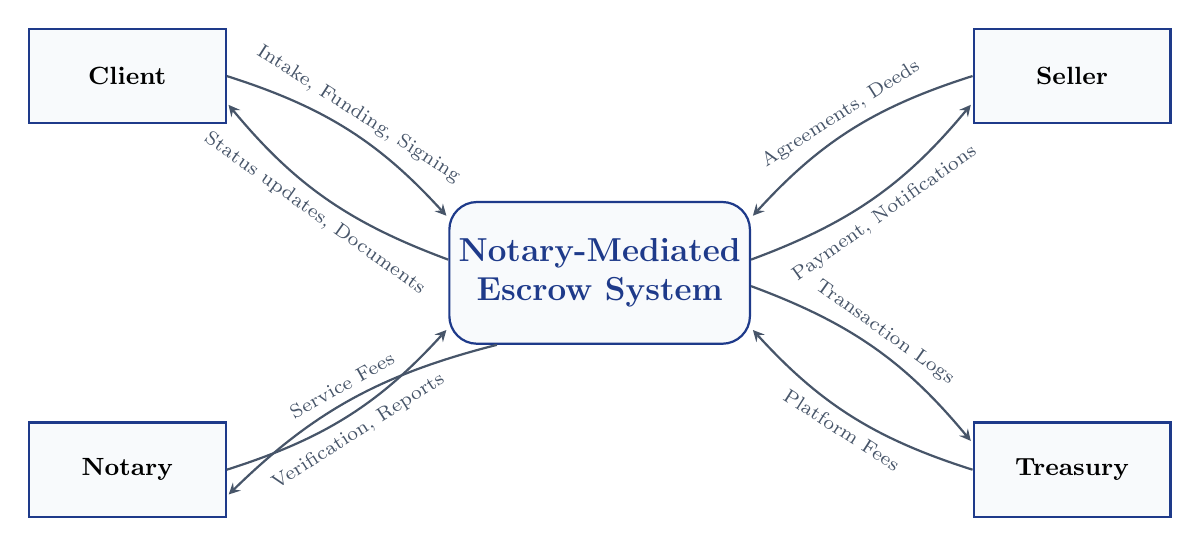
\begin{tikzpicture}[node distance=4cm, auto]
    % Central System
    \node[process] (system) at (0,0) {Notary-Mediated\\Escrow System};
    
    % External Entities
    \node[entity] (client) at (-6, 2.5) {Client};
    \node[entity] (seller) at (6, 2.5) {Seller};
    \node[entity] (notary) at (-6, -2.5) {Notary};
    \node[entity] (treasury) at (6, -2.5) {Treasury};
    
    % Client Flows (Curved to avoid overlap)
    \draw[flow] (client.0) to [bend left=15] node[above, sloped] {Intake, Funding, Signing} (system.160);
    \draw[flow] (system.175) to [bend left=15] node[below, sloped] {Status updates, Documents} (client.345);
    
    % Seller Flows
    \draw[flow] (seller.180) to [bend right=15] node[above, sloped] {Agreements, Deeds} (system.20);
    \draw[flow] (system.5) to [bend right=15] node[below, sloped] {Payment, Notifications} (seller.195);
    
    % Notary Flows
    \draw[flow] (notary.0) to [bend right=15] node[below, sloped] {Verification, Reports} (system.200);
    \draw[flow] (system.215) to [bend right=15] node[above, sloped] {Service Fees} (notary.345);
    
    % Treasury Flows
    \draw[flow] (treasury.180) to [bend left=15] node[below, sloped] {Platform Fees} (system.340);
    \draw[flow] (system.355) to [bend left=15] node[above, sloped] {Transaction Logs} (treasury.165);

\end{tikzpicture}
\end{center}

\section{Level 1 DFD}

\subsection{Process Overview}

\begin{center}
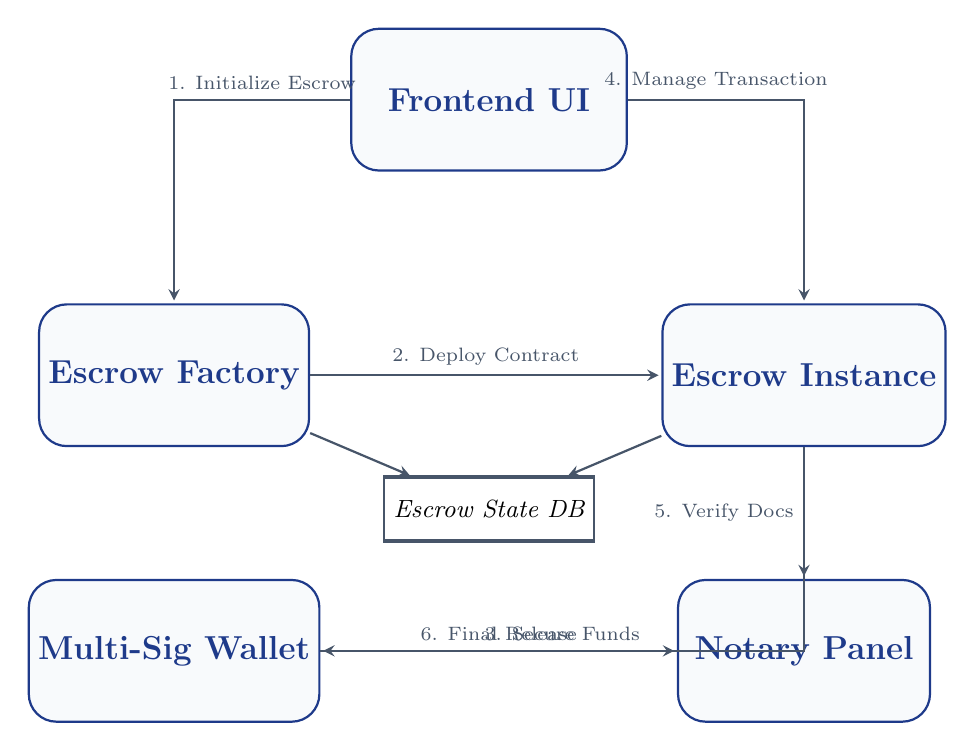
\begin{tikzpicture}[node distance=3cm, auto]
    % Level 1 Nodes
    \node[process] (frontend) at (0,4) {Frontend UI};
    \node[process, minimum width=3.2cm] (factory) at (-4,0.5) {Escrow Factory};
    \node[process, minimum width=3.2cm] (escrow) at (4,0.5) {Escrow Instance};
    \node[process, minimum width=3.2cm] (multisig) at (-4,-3) {Multi-Sig Wallet};
    \node[process, minimum width=3.2cm] (notary) at (4,-3) {Notary Panel};
    
    % Flows
    \draw[flow] (frontend) -| node[above, pos=0.25] {1. Initialize Escrow} (factory);
    \draw[flow] (factory) -- node[above] {2. Deploy Contract} (escrow);
    \draw[flow] (frontend) -| node[above, pos=0.25] {4. Manage Transaction} (escrow);
    
    \draw[flow] (escrow) -- node[left] {5. Verify Docs} (notary);
    \draw[flow] (escrow) |- node[above, pos=0.75] {3. Secure Funds} (multisig);
    \draw[flow] (multisig) -- node[above] {6. Final Release} (notary);
    
    % Data Store
    \node[datastore] (state) at (0,-1.2) {Escrow State DB};
    \draw[flow] (escrow) -- (state);
    \draw[flow] (factory) -- (state);
\end{tikzpicture}
\end{center}

\subsection{Process 1: Client Intake}

\begin{center}
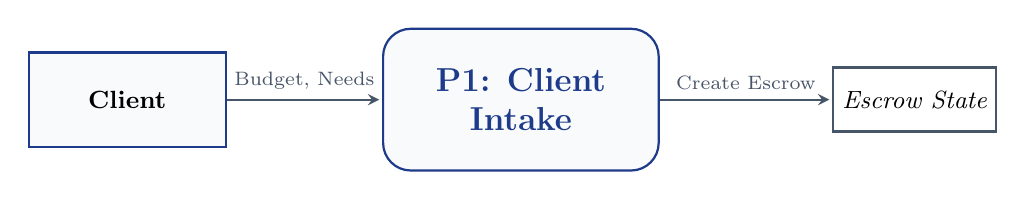
\begin{tikzpicture}[node distance=3cm, auto]
    \node[entity] (client) at (-5,0) {Client};
    \node[process] (intake) at (0,0) {P1: Client\\Intake};
    \node[datastore] (db) at (5,0) {Escrow State};
    
    \draw[flow] (client) -- node[above] {Budget, Needs} (intake);
    \draw[flow] (intake) -- node[above] {Create Escrow} (db);
\end{tikzpicture}
\end{center}

Data Elements:
\begin{itemize}
\item Input: budget, desiredSize, purpose, seller, notary
\item Output: escrowId, created event
\item Storage: EscrowTransaction struct
\end{itemize}

\subsection{Process 2: Discovery Phase}

\begin{center}

\begin{tikzpicture}[node distance=3cm, auto]
    \node[entity] (notary) at (-5,0) {Notary};
    \node[process] (discovery) at (0,0) {P2: Property\\Discovery};
    \node[datastore] (gallery) at (5,0) {Digital Gallery};
    
    \draw[flow] (notary) -- node[above] {Property Data} (discovery);
    \draw[flow] (discovery) -- node[above] {Gallery URL} (gallery);
\end{tikzpicture}
\end{center}

Data Elements:
\begin{itemize}
\item Input: geoPins, photos, videos
\item Output: gallery uploaded event
\end{itemize}

\subsection{Process 3: Due Diligence}

\begin{center}
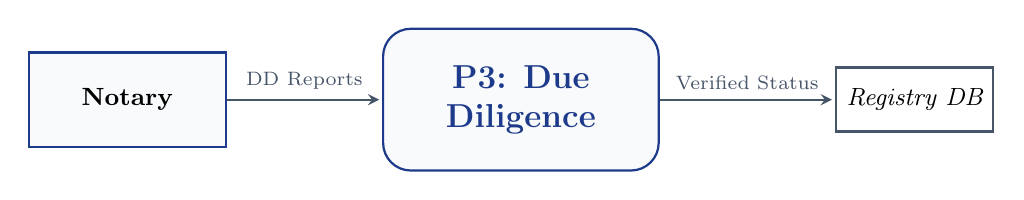
\begin{tikzpicture}[node distance=3cm, auto]
    \node[entity] (notary) at (-5,0) {Notary};
    \node[process] (dd) at (0,0) {P3: Due\\Diligence};
    \node[datastore] (registry) at (5,0) {Registry DB};
    
    \draw[flow] (notary) -- node[above] {DD Reports} (dd);
    \draw[flow] (dd) -- node[above] {Verified Status} (registry);
\end{tikzpicture}
\end{center}

Documents:
\begin{itemize}
\item SearchCertificate
\item DueDiligenceReport
\item Site Visit Report
\end{itemize}

\subsection{Process 4: Execution Phase}

\begin{center}
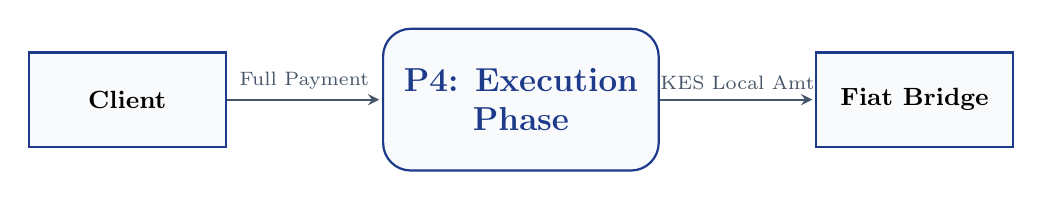
\begin{tikzpicture}[node distance=3cm, auto]
    \node[entity] (client) at (-5,0) {Client};
    \node[process] (exec) at (0,0) {P4: Execution\\Phase};
    \node[entity] (fiat) at (5,0) {Fiat Bridge};
    
    \draw[flow] (client) -- node[above] {Full Payment} (exec);
    \draw[flow] (exec) -- node[above] {KES Local Amt} (fiat);
\end{tikzpicture}
\end{center}

Flow:
\begin{enumerate}
\item Sign sale agreement
\item Notarize document
\item Client funds escrow
\item Execute fiat bridge
\item Disburse to seller
\end{enumerate}

\subsection{Process 5: Final Transfer}

\begin{center}
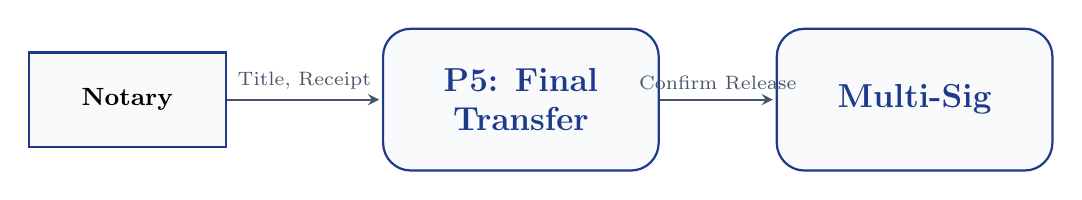
\begin{tikzpicture}[node distance=3cm, auto]
    \node[entity] (notary) at (-5,0) {Notary};
    \node[process] (transfer) at (0,0) {P5: Final\\Transfer};
    \node[process] (multi) at (5,0) {Multi-Sig};
    
    \draw[flow] (notary) -- node[above] {Title, Receipt} (transfer);
    \draw[flow] (transfer) -- node[above] {Confirm Release} (multi);
\end{tikzpicture}
\end{center}

Documents:
\begin{itemize}
\item LodgementReceipt
\item OriginalTitle
\item LCBConsent
\end{itemize}

\section{Data Stores}

\subsection{DS1: Escrow State}
\begin{itemize}
\item Stores all escrow transactions
\item Current state per escrow
\item Milestone completion status
\end{itemize}

\subsection{DS2: Documents}
\begin{itemize}
\item Document hashes per escrow
\item Verification status
\item Signing status
\end{itemize}

\subsection{DS3: Multi-Sig Wallet}
\begin{itemize}
\item Owner list
\item Pending transactions
\item Confirmation status
\end{itemize}

\section{External Interfaces}

\subsection{Ethereum Blockchain}
\begin{itemize}
\item Smart contract deployment
\item Transaction submission
\item Event logging
\item State queries
\end{itemize}

\subsection{Frontend API}
\begin{itemize}
\item Wallet connection (MetaMask)
\item Contract interaction (ethers.js)
\item Event monitoring
\item State display
\end{itemize}

\section{Flow Numbers}

\subsection{P1: Client Intake}
\begin{enumerate}
\item Client submits intake data
\item Contract validates budget $\ge$ due diligence fee
\item Escrow created with new ID
\item State set to Intake
\end{enumerate}

\subsection{P2: Property Discovery}
\begin{enumerate}
\item Notary uploads digital gallery
\item Escrow state transitions to Discovery
\item Client reviews properties
\item Client selects plot
\item State transitions to PlotSelected
\end{enumerate}

\subsection{P3: Due Diligence}
\begin{enumerate}
\item Client funds escrow with due diligence fee
\item State transitions to DueDiligencePending
\item Notary uploads DD report
\item Client verifies documents
\item State transitions to DueDiligenceComplete
\item Due diligence fee released to notary
\end{enumerate}

\subsection{P4: Execution}
\begin{enumerate}
\item Client proceeds with purchase
\item Both parties sign agreement
\item Notary notarizes document
\item Client funds remaining amount
\item Notary executes fiat bridge
\item State transitions to ExecutionComplete
\item Deposit released to seller
\end{enumerate}

\subsection{P5: Final Transfer}
\begin{enumerate}
\item Notary uploads lodgement receipt
\item State transitions to TransferRegistry
\item Notary confirms title documents
\item Multi-sig confirms final release
\item Facilitation fee to treasury
\item Balance to seller
\item State transitions to Completed
\end{enumerate}

\section{Summary}

This DFD illustrates the complete data flow through the Notary-Mediated Escrow System. Key observations:

\begin{enumerate}
\item State machine provides strict phase enforcement
\item Multi-sig protects all fund movements
\item Notary acts as trusted oracle
\item Documents hashed for immutability
\item Fiat bridge enables local currency conversion
\end{enumerate}

\vfill
\begin{center}
\textit{© 2026 Escrow Platform - Secure Land Purchase System}
\end{center}

\end{document}